\RequirePackage{plautopatch}
\RequirePackage[l2tabu, orthodox]{nag}

% \documentclass[platex,dvipdfmx]{jlreq}			% for platex
% \documentclass[platex,dvipdfmx, twocolumn]{jlreq}			% for platex
\documentclass[platex,dvipdfmx, twocolumn]{jsarticle}			% for platex
% \documentclass[uplatex,dvipdfmx]{jlreq}		% for uplatex
\usepackage{graphicx}
\usepackage{bxtexlogo}
\usepackage{braket} % ブラケット
\pagestyle{empty}

\title{初期状態が不完全な場合のグローバーアルゴリズムの振る舞いについて}

\author{東海大学理学部物理学科 伊與田研究室 9BSP1118 村岡海人}
% \date{\today}
\begin{document}
\maketitle
\section{背景と目的}
量子コンピュータとは、量子力学を利用して計算を行うコンピュータである。
この量子コンピュータで行う計算を量子計算と呼び、量子計算で扱うアルゴリズムのことを量子アルゴリズムと呼ぶ。

量子計算を行う際に、ハミルトニアンや時間がズレてしまうと実現したい操作からズレた操作を行うことになる。
また、このズレが常に発生すれば系統誤差としてみなせる。
本研究では、初期状態を準備する操作が不完全な場合に、グローバーアルゴリズムがどれだけ機能するか調べることを目的とした。

\section{基本事項}
グローバーのアルゴリズムは$N個$のデータに対して、全ての重ね合わせ状態を用意し、解の確率振幅を増幅する演算を$k$回、繰り返すことにより、$O(\sqrt{N})$回の計算量で解を見出すことができる。
古典的な探索アルゴリズムにも同じ計算量を持つ2分探索があるが、2分探索アルゴリズムは事前にソートされているデータを扱うため、ソートされていないデータの探索アルゴリズムはグローバーのアルゴリズムの方が高速である。
\cite{QuantumDojo}

アダマール演算子$H$は、量子ビットの基底状態$\ket{0},\ket{1}$の2つの重ね合わせへの写像である。
この演算子は、1量子ビットの任意の$Z-Y$回転行列に分解することができる。
本研究では、アダマール演算子$H$に$y$軸方向のズレ$\delta_y$を加えることを想定する。
\cite{BasicQuantumComputer}
% TODO:その他の状態(z軸、y,z軸)も将来書くこと

\section{研究内容と結果}
量子シミュレータQulacsを用いて、グローバーのアルゴリズムの実装を実装した。
3量子ビットのグローバーのアルゴリズムに$\delta_y$を$0$から$2\pi$まで加え、
最適な繰り返し回数$k$の解の状態の確率振幅を計算する数値実験を行い、図\ref{fig:P(k)}はその結果である。
この結果から、$\frac{\pi}{2}$を境に確率振幅が下がり、$\frac{5}{4}\pi$で極小となり、$\frac{5}{4}\pi$では解の状態の確率振幅がほとんど増加しないことを示している。

卒業研究発表では、図\ref{fig:P(k)}の詳細な説明と、その原因について発表する。

\begin{figure}
\centering
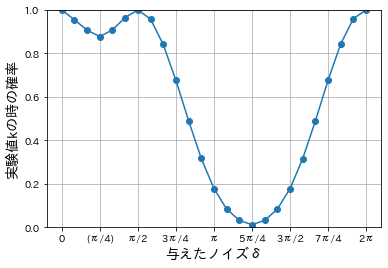
\includegraphics[width=70mm]{figures/p(k)graph.png}
\caption{ノイズ$\delta_y$を加えた時の最適な繰り返し回数の推移}
\label{fig:P(k)}
\end{figure}

\bibliographystyle{junsrt}
\bibliography{references}
\end{document}